\documentclass[a4paper,11pt,captions=tableheading,DIV=12]{scrartcl}
\pdfoutput=1
\bibliographystyle{utphys27mod}

% ----------------------------------------------------------- Packages
\usepackage{amsmath,amssymb,url,cite,slashed,cancel,booktabs,hyperref,graphicx,xspace,subcaption}
%%%UNUSED%%% \usepackage{feynmp,enumerate,multirow,wrapfig}
\renewcommand\citepunct{,\penalty1000\hskip.13emplus.1emminus.1em\relax} % no line-break in \cite
\renewcommand\thefootnote{*\arabic{footnote}}
\numberwithin{equation}{section}
% COMMENTS
\newcommand{\comment}[1]{{\textbf{\small \color{red} [#1]}}}
\newcommand{\cmark}{\ding{51}} % check mark
\newcommand{\xmark}{\ding{55}} % X mark

% MATH NOTATION
\newcommand\w[1]{_{\mathrm{#1}}}
\newcommand\vc[1]{{\boldsymbol{#1}}}
\newcommand\dd{\mathop{}\!\mathrm{d}}
\newcommand\DD{\mathop{}\!\mathrm{D}}
\newcommand\ee{\mathop{}\!\mathrm{e}}
\newcommand\abs[1]{\lvert#1\rvert}
\newcommand\norm[1]{\lVert#1\rVert}
\newcommand\Abs[1]{\left\lvert#1\right\rvert}
\newcommand\Norm[1]{\left\lVert#1\right\rVert}
\newcommand\ii{\mathrm{i}}
\newcommand\co[1]{\mathrm{c}_{#1}}
\newcommand\si[1]{\mathrm{s}_{#1}}
\newcommand\coco[1]{\mathrm{c}^2_{#1}}
\newcommand\sisi[1]{\mathrm{s}^2_{#1}}
\newcommand\pmat[1]{\begin{pmatrix}#1\end{pmatrix}}
\DeclareMathOperator{\Order}{\mathcal{O}}
\DeclareMathOperator{\sign}{\mathrm{sign}}
\DeclareMathOperator{\ddelta}{\delta}
\DeclareMathOperator{\Tr}{\mathrm{Tr}}
\DeclareMathOperator{\diag}{\mathrm{diag}}

\newcommand\oneone{1}
\newcommand{\dn}[3]{\frac{\dd^#1 #2}{\dd #3^#1}}    % derivatives
\newcommand{\pdn}[3]{\frac{\partial^#1 #2}{\partial #3^#1}}
\newcommand{\pd}[2]{\frac{\partial #1}{\partial #2}}
\newcommand\paren[3]{\def\temp{#3}\Bigl(\frac{#1}{#2}\Bigr)\ifx\oneone\temp\relax\relax\else^{#3}\fi}
\newcommand\vev[1]{\langle#1\rangle}
\newcommand{\mean}[1]{\left\langle #1 \right\rangle}

\newcommand\hc{\text{h.c.}}

% units
\newcommand\unit[1]{\,\mathrm{#1}\xspace}
\newcommand\eV{\unit{eV}}
\newcommand\keV{\unit{keV}}
\newcommand\MeV{\unit{MeV}}
\newcommand\GeV{\unit{GeV}}
\newcommand\TeV{\unit{TeV}}
\newcommand\PeV{\unit{PeV}}
\newcommand\fb{\unit{fb}}
\newcommand\pb{\unit{pb}}
\newcommand\iab{\unit{ab^{-1}}}
\newcommand\ifb{\unit{fb^{-1}}}
\newcommand\ipb{\unit{pb^{-1}}}
\newcommand\fm{\unit{fm}}

% scientific form of numbers
\makeatletter
\def\EE{\@ifnextchar-{\@@EE}{\@EE}}
\def\@EE#1{\ifnum#1=1 \times\!10 \else \times\!10^{#1}\fi}
\def\@@EE#1#2{\times\!10^{-#2}}
\makeatother

% ---------------------------------------------------- For Sho's Notes
\usepackage{scrlayer-scrpage,color,soul}
\usepackage[hhmmss]{datetime}
\newdateformat{mydate}{\THEDAY\;\shortmonthname.\;\THEYEAR}
\addtokomafont{pagehead}{\small\normalfont}
\ohead{\texttt{[\jobname~@~\mydate\today~\currenttime]}}
\bibliographystyle{utphys27mod}
\newcommand{\TODO}[1]{{\textbf{\color{red}$\clubsuit$#1}}}
\newcommand{\trans}{^{\mathrm T}}
\newcommand{\spmat}[1]{\left(\begin{smallmatrix}#1\end{smallmatrix}\right)}
\renewcommand{\Re}{\mathop{\mathrm{Re}}}
\renewcommand{\Im}{\mathop{\mathrm{Im}}}
\newcommand\mtot{m_{\mathrm{tot}}}
\let\oln\overline
\newcommand\yydag{(yy^\dagger)}

\author{Sho Iwamoto}
\title{Analysis of NuFIT Best-fit points}
\begin{document}
%\maketitle
\begin{center}{\makeatletter
{\huge\usekomafont{title}\@title}\par\vspace{2em}
{\Large \@author}\par\vspace{2em}
}
\end{center}

%---------------------------------------------------------------------
\section{Notation}
\paragraph{Masses}
We introduce the following notations on the two heavier neutrino masses\footnote{We can safely neglect the differences between $M_I$ and the (diagonalized) Majorana masses.} $M_I$ and the three lighter neutrino masses $m_i$, one of which is zero, as
\begin{align*}
 \Delta M & := M_2-M_1 > 0 &
 \delta M & := \Delta M/M_1\\
 \Delta M^2 & := M_2^2-M_1^2 &
 \delta M^2 & := \Delta M^2 / M_1^2 \\
 \Delta m & := m\w{heavier} - m\w{lighter}&
 \rho_m   & := \Delta m/\mtot,&
 &\qquad \mtot    := \sum_i m_i,\\
 m\w{heavier} &= m_3~(m_2),&
 m\w{lighter} &= m_2~(m_1)& &\text{for NH~(IH).}
\end{align*}
Numerically, for BFP of NH (IH), $\rho_m\simeq\sqrt{0.5}~(0.0075)$ and $\mtot\simeq5.9~(9.9)\EE{-11}\GeV$.

\paragraph{Yukawa}
Yukawa matrix follows the notation of 1611 paper, and the CIP is given by
\begin{equation}
 y = \ii(v/\sqrt{2})^{-1}\sqrt{M\w{diag}}R\sqrt{m\w{diag}}U^\dagger
\end{equation}
with $v=\sqrt\vev{\phi_0}\approx246\GeV$,
\begin{align}
 R&=\pmat{0 & +\co z & \zeta \si z \\ 0 & -\si z & \zeta\co z}\quad\text{for NH},&
 R&=\pmat{+\co z & \zeta \si z & 0 \\ -\si z & \zeta\co z & 0}\quad\text{for IH}.
\end{align}
Here, $z\in\mathbb C$ and $\zeta=\pm1$:
\begin{equation}
 z = w + \ii x;\qquad w\in\mathbb R,\quad x\in\mathbb R,
\end{equation}
and $U=U\w{PMNS}$ follows 1611 paper, i.e., PDG with a phase matrix $\diag(1, \ee^{\ii\sigma}, 1)$.

\paragraph{Yukawa products}
We define
\begin{align*}
 W_1 = W_{11} &= \cosh2x -\rho_m\cos2w,&
 W_{12} &= W_{21}^* = \ii\sinh2x + \rho_m\sin2w,\\
 W_2 = W_{22} &= \cosh2x +\rho_m\cos2w,&
 \mu_I  &= \frac{\mtot M_I}{8\pi v^2}\approx 3.9~(6.5)\EE{-17}M_I/\text{GeV},
\end{align*}
for NH (IH), which leads us to
\begin{align}
 \yydag_{IJ} &= \frac{\mtot\sqrt{M_IM_J}}{v^2}W_{IJ},&
 \Gamma_{I} &= \frac{\yydag_{II}}{8\pi}M_I = \mu_I W_I M_I.
\end{align}

\paragraph{Effective neutrino masses}
Remembering that $m_i$ is given by
\begin{equation}
 m_i = \left[U\trans\left(-\frac{v^2}{2}y\trans M^{-1} y\right)U\right]_{ii}
     = U_{i\alpha}\left(-\frac{v^2}{2}\sum_I \frac{y_{I\alpha}  y_{I\beta}}{M_I}\right)U_{\beta i},
\end{equation}
we define
\begin{align}
 \widetilde{m_I} &:= \frac{v^2}{2}\sum_\alpha \frac{  \abs{y_{I\alpha}}^2}{M_I}
                  = \frac{v^2}{2}\frac{\yydag_{II}}{M_I},
&
 m_* := 1.66\sqrt{g_*}\frac{8\pi (v^2/2)}{M\w{pl}}\sim 1\EE-{12}\GeV.
\end{align}
Note that these effective neutrino masses are related to
\begin{equation}
 \widetilde{m_I} = \frac{\mtot}{2}W_I.
\end{equation}

\section{Neutrino-option condition}
The neutrino-option condition is given by, matching at $Q_0=M_1\ee^{-3/4}$,
\begin{equation}
 \mu^2\w{EFT}(Q_0)
= \frac{M_1^2}{16\pi^2}\Tr\yydag.
\end{equation}
Defining
\begin{equation}
 f(M_1) := \frac{8\pi^2v^2\cdot\mu^2\w{EFT}(Q_0)}{M_1^3}\Big|_{Q=M_1\exp(-3/4)},
\end{equation}
we can rewrite the neutrino-option condition as
\begin{equation}
f(M_1)
 =
\frac{v^2}{2}\frac{\Tr\yydag}{M_1}.
\end{equation}
The right-hand side is parameterized as\footnote{Notice that
$\cosh2x = (\widetilde{m_1}+\widetilde{m_2})/\mtot$, where $\widetilde{m_I}$ is an effective neutrino parameter.}
\begin{equation}
\frac{v^2}{2}\frac{\Tr\yydag}{M_1}
= \mtot\left[\cosh2x + \frac{\delta M}{2}(\cosh2x+\rho_m\cos2w)\right] > \mtot.
\end{equation}



Therefore, the neutrino-option condition gives a constraint
\begin{equation}
 f(M_1) > \mtot.
\end{equation}
This is translated to an upper bound on $M_1$, which is
\begin{equation}
 M_1<9.4\ (7.9)\times10^6\GeV\quad\text{for NH (IH)}
\end{equation}
Meanwhile, for $M_1$ below this upper bound, we can always find a solution to the neutrino-option condition. With small $\delta M$,
\begin{equation}
 \cosh2x\simeq \frac{f(M_1)}{\mtot}.
\end{equation}
For example, for $M_1=4$ (1) $\times10^6\GeV$, the condition is satisfied with $\cosh2x \sim 10$ (1000).


\section{Leptogenesis}
The resulting lepton asymmetry is approximately given by
\begin{equation}
  \delta \eta_l\simeq
\sum_{\alpha}\frac{\sum_I\epsilon_{I\alpha}}{D_\alpha},
\end{equation}
where
\begin{align}
  \epsilon_{I\alpha} &= F_{I\alpha}f^{\mathrm{vertex}}_{IJ}+\left(
F_{I\alpha} + \frac{M_I}{M_J}F'_{I\alpha}
\right)(f^{\mathrm{osc}}_{IJ} + f^{\mathrm{mix}}_{IJ}),
&
  D_\alpha &:= K_\alpha^{\text{eff}}\min(z_c, z_\alpha).
\end{align}

For the numerator, we introduced
\begin{align*}
 F_{I\alpha} &:= \frac{\Im\left[y_{I\alpha}y^*_{J\alpha}(y y^\dagger)_{IJ}\right]}
{(y y^\dagger)_{II}(y y^\dagger)_{JJ}}\Bigg|_{J=3-I},
&
 F'_{I\alpha} &:= \frac{\Im\left[y_{I\alpha}y^*_{J\alpha}(y y^\dagger)_{JI}\right]}
{(y y^\dagger)_{II}(y y^\dagger)_{JJ}}\Bigg|_{J=3-I},
\end{align*}
\begin{align*}
 f^{\text{vertex}}_{IJ}
&:= \frac{\Gamma_J}{M_I}
\left[1-\left(1+\frac{M_J^2}{M_I^2}\right)\ln\left(1+\frac{M_I^2}{M_J^2}\right)\right],
&
 f^{\text{mix}}_{IJ}
&:= \frac{R_{IJ}}
         {1+R_{IJ}^2},&
 f^{\text{osc}}_{IJ}
&:= \frac{R_{IJ}}
         {1+\rho\w{osc} R_{IJ}^2},
\end{align*}
\begin{align*}
  R_{IJ} &:= \frac{M_I\Gamma_J}{M_I^2-M_J^2},
&
 \rho\w{osc} &
= \left(\frac{M_J}{M_I} + \frac{\Gamma_I}{\Gamma_J}\right)^2
\frac{\det\left[\Re(yy^\dagger)\right]}{(yy^\dagger)_{11}(yy^\dagger)_{22}}.
\end{align*}
while, for the denominator,
\begin{align*}
 z_\alpha &= 1.25\log25 K_\alpha^{\mathrm{eff}},&
 z_c &= \frac{M_1}{149\GeV},
&
 K_\alpha^{\mathrm{eff}}
&= \kappa_\alpha \sum_I \frac{\Gamma_I}{H_N}\frac{|y_{I\alpha}|^2}{(yy^\dagger)_{II}}.
\end{align*}

\subsection{Numerator}
In this subsection, we assume
\begin{itemize}
 \item the contribution from vertex corrections is negligible,
 \item $\mu_1, \mu_2 \ll \delta M \ll 1$,
\end{itemize}
which we should discuss elsewhere (but SI checks the validity).
Due to the second assumption, we expand the expressions in terms of $\mu_I$, not of $\delta M$.

The numerator is simplified as
\begin{align}
  \sum_I\epsilon_{I\alpha}
\simeq
  \sum_I\epsilon^{\cancel{\text{vertex}}}_{I\alpha}
=
\left(
F_{I\alpha} + \frac{M_I}{M_J}F'_{I\alpha}
\right)(f^{\mathrm{osc}}_{IJ} + f^{\mathrm{mix}}_{IJ}),
\end{align}
and, defining
\begin{align}
 f_{IJ}&:=f_{IJ}^{\mathrm{mix}} + f_{IJ}^{\mathrm{osc}},
&
 F^{\pm}_\alpha &:= (F_{2\alpha}+F'_{2\alpha})\pm(F_{1\alpha}+F'_{1\alpha}),
\end{align}
we evaluate
\begin{align}
 \sum_I\epsilon^{\cancel{\text{vertex}}}_{I\alpha}
&=
\left(
F_{I\alpha} + \frac{M_I}{M_J}F'_{I\alpha}
\right)(f^{\mathrm{osc}}_{IJ} + f^{\mathrm{mix}}_{IJ}).
\\&=
\frac{f_{21}-f_{12}}{2}F_\alpha^-
+ \left(\frac{M_1-M_2}{M_2}F'_{1\alpha}f_{12} + \frac{M_2-M_1}{M_1}F'_{2\alpha}f_{21}\right),
\end{align}
where we used $F_\alpha^+=0$.
Expanding in terms of $\mu_I$ (but not in $\delta M$),
\begin{align}
\begin{split}
  \sum_I\epsilon^{\cancel{\text{vertex}}}_{I\alpha}
 &=
  \left[
 \frac{M_1 M_2}{M_2^2-M_1^2}(W_1\mu_1+W_2\mu_2) + \Order(\mu_I^3)
  \right]F^-_{\alpha}\\
 &\qquad+
\left(
\frac{2M_1\mu_2W_2F'_{1\alpha} + 2M_2\mu_1W_1F'_{2\alpha}}{M_1+M_2} + \Order(\mu_I^3)
\right).
\end{split}\label{eq:1}
\end{align}

The remaining parts are evaluated as
\begin{align}
 F^-_\alpha
&=
\frac{4\Re\yydag_{12}\Im(y_{1\alpha}^*y_{2\alpha})}{\yydag_{11}\yydag_{22}}
\\&=
\frac{4 \Re W_{12}}{W_1 W_2}\Im\left[
  \frac{2}{\mtot}
  \sum_{ij}
  R_{2i}\sqrt{m_i}(U^\dagger)_{i\alpha} U_{\alpha j}\sqrt{m_j}(R^\dagger)_{j1}
  \right]
\\&=
\frac{4 \Re W_{12}}{W_1 W_2}\left(G_\alpha^{(2)}\zeta\cosh2x - G_\alpha^{(1)}\sinh2x\right),
\end{align}
where
\begin{align}
  G^{(1)}_\alpha
&= \sum_i \frac{m_i}{\mtot}\Abs{U_{\alpha i}}^2,
&
  G^{(2)}_\alpha
&=
\begin{cases}
\left({2\sqrt{m_2m_3}}/{\mtot}\right)\Im\left(U_{\alpha2}U^*_{\alpha3}\right) & \text{(NH)}\\
\left({2\sqrt{m_1m_2}}/{\mtot}\right)\Im\left(U_{\alpha1}U^*_{\alpha2}\right) & \text{(IH)}
\end{cases}
\end{align}
Note that $G_\alpha^{(1)}\ge \abs{G_\alpha^{(2)}} \ge 0$.
Also, for the sub-leading term,
\begin{align}
 F'_{I\alpha}
&=
\frac{2}{\mtot}\sum_{i,j}
\frac{\Im\left[W_{JI}\cdot
R_{Ii}\sqrt{m_i}(U^\dagger)_{i\alpha}U_{\alpha j}\sqrt{m_j}(R^\dagger)_{jJ}
 W_{JI}\right]}
{W_1 W_2},
\end{align}
which however is not used hereafter.

\subsection{Denominator}
Now we are to evaluate
\begin{align}
 K_\alpha^{\mathrm{eff}}
= \kappa_\alpha \sum_I \frac{\Gamma_I}{H_N}\frac{|y_{I\alpha}|^2}{(yy^\dagger)_{II}}
=
\frac{\kappa_\alpha}{8\pi H_N} \sum_I \frac{2M_I^2}{v^2}\sum_{i,j}\left[
R_{Ii}\sqrt{m_i}(U^\dagger)_{i\alpha}U_{\alpha j}\sqrt{m_j}(R^\dagger)_{jI}
\right],
\end{align}
where we can assume $M_1\simeq M_2$ since $\mu_I$ does not appear in this expression.
Hence,
\begin{align}
 K_\alpha^{\mathrm{eff}}
&\approx
\frac{\kappa_\alpha}{8\pi H_N} \frac{2M_1^2}{v^2}\sum_{I,i,j}\left[
R_{Ii}\sqrt{m_i}(U^\dagger)_{i\alpha}U_{\alpha j}\sqrt{m_j}(R^\dagger)_{jI}
\right]\\
&=
\frac{\kappa_\alpha}{8\pi H_N} \frac{2M_1^2}{v^2}\sum_{i,j}\left[
U_{\alpha j}\sqrt{m_j}(R^\dagger R)_{ji}\sqrt{m_i}(U^\dagger)_{i\alpha}
\right]
\\&=
\frac{\kappa_\alpha \mtot}{m_*}
\left(
G_\alpha^{(1)}\cosh2x - G_\alpha^{(2)}\zeta\sinh2x
\right).
\end{align}
\TODO{Here some $\zeta(3)$ is missing; readers should amend it.}


\subsection{Result}
We now have a simple analytic expression for $\delta \eta_l$ under the assumptions
\begin{itemize}
 \item vertex contribution is negligible,
 \item $\mu_1, \mu_2 \ll \delta M \ll 1$,
 \item the term in the second line of Eq.~\ref{eq:1} is negligible:
\end{itemize}
with $z_*=\min(z_c,z_\alpha)$, \TODO{$\zeta(3)$ should be included}
\begin{align}
  \delta \eta_l
&\simeq
-\sum_\alpha \frac1{\kappa_\alpha z_*}
\frac{M_1M_2}{M_2^2-M_1^2}
\frac{m_*}{\mtot}
\frac{4(W_1 \mu_1 + W_2 \mu_2)\Re W_{12}}{W_1W_2}
\frac{G_\alpha^{(1)}\tanh2x-\zeta G_\alpha^{(2)}}
{G_\alpha^{(1)}-\zeta G_\alpha^{(2)}\tanh2x}
\\&=
-\sum_\alpha \frac1{\kappa_\alpha z_*}
\frac{M_2}{M_2-M_1}
\frac{m_* M_1}{8\pi v^2}
\frac{4\rho_m\cosh2x\sin2w}{\cosh^22x-\rho_m^2\cos^22w}
\left(1+\frac{\rho_m\cos2w}{2\cosh2x}\delta'M\right)
G_\alpha,\label{eq:2}
\end{align}
where $\delta'M:=2\Delta M/(M_1+M_2)\simeq\delta M$.
Here, the PMNS-matrix dependence is contained in
\begin{equation}
 G_\alpha :=
\frac{G_\alpha^{(1)}\tanh2x-\zeta G_\alpha^{(2)}}
{G_\alpha^{(1)}-\zeta G_\alpha^{(2)}\tanh2x}.
\end{equation}



\section{(a few) Discussion}
\subsection{Hierarchy}
Let us evaluate the factors $G_\alpha^{(a)}$ at the NuFIT~4.0 best-fit points.
For normal hierarchy,
\begin{align*}
 G_\alpha^{(1)} &= \pmat{0.0634\\0.535\\0.401},
&
 G_\alpha^{(2)} &= \pmat{
  -0.0334 & -0.0477\\
  +0.0194 & +0.314\\
  +0.0140 & -0.266
}\pmat{\cos\sigma\\\sin\sigma},
&
 \pmat{\rho_m\\\mtot}&=\pmat{0.708 \\ 5.89\EE-2\eV}
\end{align*}
and for inverted hierarchy,
\begin{align*}
 G_\alpha^{(1)} &= \pmat{0.487\\0.215\\0.298},
&
 G_\alpha^{(2)} &= \pmat{
   0      & -0.452\\
  +0.0720 & +0.193\\
  -0.0720 & +0.259
}\pmat{\cos\sigma\\\sin\sigma},
&
 \pmat{\rho_m\\\mtot}&=\pmat{0.00746 \\ 9.95\EE-2\eV}.
\end{align*}
Note that the leptogenesis works better in normal hierarchy due to the larger $\rho_m$,

\begin{figure}[ht]
  \centering
  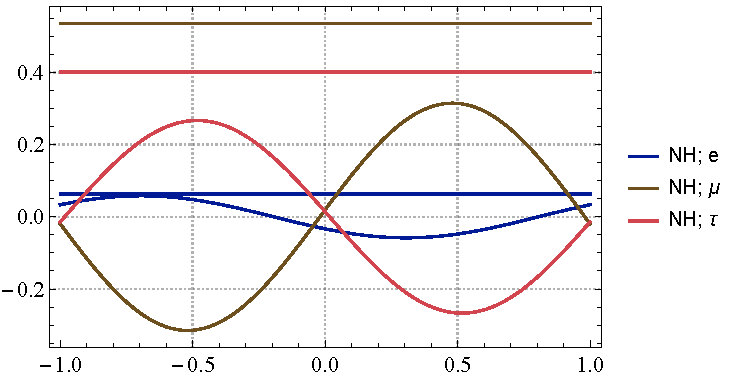
\includegraphics[width=0.49\textwidth]{bfp_analysis_f_NH.pdf}
  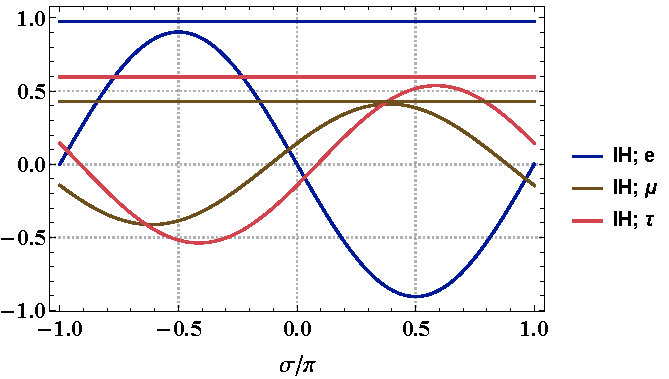
\includegraphics[width=0.49\textwidth]{bfp_analysis_f_IH.pdf}
\end{figure}

\subsection{Strict lower bound}
Let us derive an analytic upper bound $\overline{\delta \eta_l}$, where the absolute value of analytic expression \eqref{eq:2} is always smaller than it.
Since $\sin2w/(\cosh^22x-\rho_m^2\cos^22w)$ is maximal for $w=\pi/4$,
\begin{align}
  \overline{\delta \eta_l}
&=
\frac1{z_*}
\frac{M_2}{M_2-M_1}
\frac{m_* M_1}{8\pi v^2}
\frac{4\rho_m}{\cosh2x}
\left(1+\frac{\rho_m\cos2w}{2\cosh2x}\delta'M\right)
\sum_\alpha\frac{G_\alpha}{\kappa_\alpha},
\\&=
\frac1{z_*}
\frac{M_2}{M_2-M_1}
\frac{2.81M_1\rho_m}{10^{18}\GeV\cdot\cosh2x}
\left(1+\frac{\rho_m\cos2w}{2\cosh2x}\delta'M\right)
\sum_\alpha\frac{G_\alpha}{\kappa_\alpha}.
\end{align}
Thus, assuming $M_1\gg10^{10}\GeV$, we require $\delta M\ll 1$:
\begin{equation}
 \overline{\delta \eta_l}
\simeq
\frac1{z_*\delta M}
\frac{2.81M_1\rho_m}{10^{18}\GeV}
\sum_\alpha\frac{G_\alpha}{\kappa_\alpha\cosh2x}.
\end{equation}
We can numerically maximize $\sum_\alpha G_\alpha/\cosh2x$ for $x$; around the best-fit point, its maximum value is $\sim1.5$ for both hierarchies.
Therefore, to get $\delta\eta_l\sim3\EE-8$, we need
\begin{equation}
 \frac{M_1}{\delta M}\sim 2\EE{10}\GeV ~~(2\EE{12}\GeV)
\end{equation}
for NH (IH) if $G_\alpha$ has no special cancellation.


\subsection{With neutrino option}
In Section 2, we saw that the neutrino-option condition is satisfied even for smaller $M_1$ with huge $\cosh2x$:
\begin{equation}
 \cosh2x\simeq \frac{f(M_1)}{\mtot} = \frac{8\pi^2v^2\mu^2\w{EFT}(Q_0)}{M_1^3\mtot}\approx
\frac{4.8\EE{10}\GeV^4}{M_1^3\mtot}
\end{equation}
This equality is precise for smaller $\delta M$, which we need to have an adequate $\delta \eta_l$:
\begin{equation}
 \overline{\delta \eta_l}
\simeq
\frac{3\EE-8}{z_*}
\left(\frac{M_1/(\delta M)^{1/4}}{5.9\EE7\GeV~~(1.6\EE8\GeV)}\right)^4
\sum_\alpha\frac{G_\alpha}{\kappa_\alpha}\Big|_{\text{$\cosh2x$ for n.o.}}.
\end{equation}

Or, using the upper-bound value of $M_1$,
\begin{equation}
  \overline{\delta \eta_l}
\simeq
\frac{3\EE-8}{z_*}
\left(\frac{M_1}{9.4\EE6\GeV}\right)^4\frac{6.3\EE-4}{\delta M}
\sum_\alpha\frac{G_\alpha}{\kappa_\alpha}\Big|_{\text{$\cosh2x$ for n.o.}}.
\end{equation}
for NH and
\begin{equation}
  \overline{\delta \eta_l}
\simeq
\frac{3\EE-8}{z_*}
\left(\frac{M_1}{7.9\EE6\GeV}\right)^4\frac{5.6\EE-6}{\delta M}
\sum_\alpha\frac{G_\alpha}{\kappa_\alpha}\Big|_{\text{$\cosh2x$ for n.o.}}.
\end{equation}
for IH; therefore, for IH, we need a special cancellation in $\delta M$ or $G_\alpha$.\footnote{
One may also notice that $G_\alpha\to 1$ for $\cosh 2x\gg 1$.
}


\appendix
\section{Leptogenesis with smaller mass splitting}
In Section 3.1 we assume $\mu_I\ll\delta M\ll 1$ and expand the formulae in terms of $\mtot$, or take a limit of $R_{IJ}\ll 1$:
\begin{equation}
 R_{IJ}\simeq \frac{\mu_J W_J}{2\delta M} \ll 1.
\end{equation}
For $\delta M\ll \mu_I$, we instead should expand the formulae with $R_{IJ}\gg1$.
Then,
\begin{equation}
 \sum_I \epsilon^{\cancel{\text{vertex}}}_{I\alpha}
\approx
\frac{f_{21}-f_{12}}{2}
F_\alpha^-,
\end{equation}
where
\begin{align}
\frac{f_{21}-f_{12}}{2}
\approx
\frac{\delta M}{\mu_1}
\left(
\frac{W_1 W_2}{2\cosh2x(\cosh^2 2x - \rho_m^2)} + \frac{2\cosh2x}{W_1 W_2}
\right).
\end{align}
Denominator is calculated as before, and the asymmetry is given by
\TODO{$\zeta(3)$ should be included}
\begin{align}
\delta\eta_l
&\approx
-\sum_\alpha
\frac{8\pi v^2 m_* \delta M}{z_* \kappa_\alpha \mtot^2 M_1}
\left(
\frac{W_1 W_2}{2\cosh2x(\cosh^2 2x - \rho_m^2)} + \frac{2\cosh2x}{W_1 W_2}
\right)
\frac{4\Re W_{12}}{W_1 W_2}
G_\alpha
\\
&=-\sum_\alpha
\frac{8\pi v^2 m_* \delta M}{z_* \kappa_\alpha \mtot^2 M_1}
\left(
\frac{W_1 W_2}{2\cosh2x(\cosh^2 2x - \rho_m^2)} + \frac{2\cosh2x}{W_1 W_2}
\right)
\frac{4\sin2w}{W_1 W_2}
G_\alpha,
\end{align}
where $W_1 W_2 = \cosh^2 2x - \rho_m^2\sin^22w$.
The asymmetry is maximized with $w=\pi/4$;
\begin{equation}
\overline{\delta\eta_l}
=\sum_\alpha
\frac{16\pi v^2 m_* \delta M}{z_* \kappa_\alpha \mtot^2 M_1}
\frac{5\cosh^2 2x - \rho_m^2}{\left(\cosh^2 2x - \rho_m^2\right)^2\cosh2x}
G_\alpha.
\end{equation}

\newpage
\section{Appendix for kappa}
We evaluate the expressions in our draft,
\begin{equation}
\kappa_\alpha = 2\sum_{I,J} \frac{\textrm{Re}\big[y_{I\alpha}^{\phantom{*}}y_{J\alpha}^*\big]\textrm{Re}\left[\left(yy^\dagger\right)_{IJ}\right] - \textrm{Im}\big[y_{I\alpha}^{\phantom{*}}y_{J\alpha}^*\big]\textrm{Im}\big[y_{I\alpha}^{\phantom{*}}y_{J\alpha}^*\big]}{\left(y^\dagger y\right)_{\alpha\alpha}\left[\left(yy^\dagger\right)_{II} + \left(yy^\dagger\right)_{JJ}\right]}\left(1-2\ii\,\frac{M_I-M_J}{\Gamma_I+\Gamma_J}\right)^{-1}.
\end{equation}
We get
\begin{align}
\begin{split}
 \kappa_\alpha
 &= 2\sum_{I} \frac{
  |y_{I\alpha}|^2
  \Re(yy^\dagger)_{II}
  }{\left(y^\dagger y\right)_{\alpha\alpha}\cdot 2(yy^\dagger)_{II}}
 \\&\qquad+
 2 \frac{\Re[y_{1\alpha} y_{2\alpha}^*]\Re[(yy^\dagger)_{12}] - [\Im(y_{1\alpha}y_{2\alpha}^*)]^2
}{(y^\dagger y)_{\alpha\alpha}\left[\yydag_{11} + \yydag_{22}\right]}
\left(1-2\ii\frac{M_1-M_2}{\Gamma_1+\Gamma_2}\right)^{-1}
 \\&\qquad+
 2 \frac{\Re[y_{2\alpha} y_{1\alpha}^*]\Re[(yy^\dagger)_{21}] - [\Im(y_{2\alpha}y_{1\alpha}^*)]^2
}{(y^\dagger y)_{\alpha\alpha}\left[\yydag_{11} + \yydag_{22}\right]}
\left(1-2\ii\frac{M_2-M_1}{\Gamma_1+\Gamma_2}\right)^{-1}
\end{split}
\\
\begin{split}
 &= 1 + 
 2 \frac{\Re[y_{1\alpha} y_{2\alpha}^*]\Re[(yy^\dagger)_{12}] - [\Im(y_{1\alpha}y_{2\alpha}^*)]^2
}{(y^\dagger y)_{\alpha\alpha}\left[\yydag_{11} + \yydag_{22}\right]}
\\&\qquad\qquad\times
\left[
\left(1-2\ii\frac{M_1-M_2}{\Gamma_1+\Gamma_2}\right)^{-1}
+
\left(1-2\ii\frac{M_2-M_1}{\Gamma_1+\Gamma_2}\right)^{-1}
\right]\end{split}
\\&=
 1 + 
 2 \frac{\Re[y_{1\alpha} y_{2\alpha}^*]\Re[(yy^\dagger)_{12}] - [\Im(y_{1\alpha}y_{2\alpha}^*)]^2
}{(y^\dagger y)_{\alpha\alpha}\left[\yydag_{11} + \yydag_{22}\right]}
\frac{2(\Gamma_1+\Gamma_2)^2}{(\Gamma_1+\Gamma_2)^2+4(\Delta M)^2}.
\end{align}
Now we should explicitly evaluate the Yukawa products.

Let us define
\begin{align}
 g_{\alpha i} &:= \frac{m_i}{\mtot}\Abs{U_{\alpha i}}^2,
&
 h_{\alpha} &:= 
\begin{cases}
\left({2\sqrt{m_2m_3}}/{\mtot}\right)\left(U_{\alpha2}U^*_{\alpha3}\right) & \text{(NH)}\\
\left({2\sqrt{m_1m_2}}/{\mtot}\right)\left(U_{\alpha1}U^*_{\alpha2}\right) & \text{(IH)}
\end{cases}
\end{align}
which leads
\begin{align}
 G^{(1)}_\alpha &= \sum_i g_{\alpha i},
&
 G_\alpha^{(2)} &= \Im h_\alpha.
\end{align}
Then we evaluate the Yukawa product as
\begin{align}
 y_{I\alpha} y^*_{J\alpha}
&=
\frac{1}{v^2/2}
\sqrt{M_I M_J}(R\sqrt{m\w{diag}}U^\dagger)_{I\alpha}(U\sqrt{m\w{diag}}R^\dagger)_{\alpha J}
\\&=
\frac{1}{v^2/2}\sum_{i,j}
U_{\alpha i}U^*_{\alpha j}
(\sqrt{m\w{diag}}R^\dagger)_{i J}
\sqrt{M_I M_J}
(R\sqrt{m\w{diag}})_{Ij}
\\&=
\frac{\mtot\sqrt{M_I M_J}}{v^2/2}
\left[
   \sum_{i}R_{Ii}g_{\alpha i}(R^\dagger)_{iJ}
   +\frac12\left(
      h_\alpha   R^*_{J2} R_{I3}+
      h_\alpha^* R^*_{J3} R_{I2}
   \right)
\right].
\end{align}
For inverted hierarchy, we just replace the indices as usual.
Then we get
\begin{align}
 \Re\left(y_{1\alpha} y^*_{2\alpha}\right)
&=
\frac{\mtot\sqrt{M_1 M_2}}{v^2}
\Bigl[
(g_{\alpha 3}-g_{\alpha2})\sin2w
+(\Re h_\alpha)\zeta\cos2w\Bigr],\\
 \Im\left(y_{1\alpha} y^*_{2\alpha}\right)
&=
\frac{\mtot\sqrt{M_1 M_2}}{v^2}
\Bigl[
(g_{\alpha 3}+g_{\alpha2})\sinh2x
 - (\Im h_\alpha)\zeta\cosh2x
\Bigr],
\end{align}
which leads
\begin{align}
& \frac{\Re[y_{1\alpha} y_{2\alpha}^*]\Re[(yy^\dagger)_{12}] - [\Im(y_{1\alpha}y_{2\alpha}^*)]^2
}{(y^\dagger y)_{\alpha\alpha}\left[\yydag_{11} + \yydag_{22}\right]}
\\&=
 \frac{\left[
(g_{\alpha 3}-g_{\alpha2})\sin2w
+(\Re h_\alpha)\zeta\cos2w\right]
\Re W_{12} - \left(G_\alpha^{(1)}\sinh2x-\zeta G^{(2)}_\alpha\cosh2x\right)^2
}{\frac{v^2}{\mtot M_1 M_2}(y^\dagger y)_{\alpha\alpha} (M_1W_1+M_2W_2)},
\end{align}
and, for $M_1\simeq M_2$,
\begin{align}
 (y^\dagger y)_{\alpha\alpha}
&\simeq
\frac{2M_1\mtot}{v^2}\left(
  G^{(1)}_\alpha\cosh2x - \zeta G^{(2)}_\alpha\sinh2x
\right).
\end{align}

\end{document}
